\documentclass[12pt, a4paper]{article}

\usepackage{parskip}
\usepackage{titling}
\usepackage{float}
\usepackage{pgf-pie}

% Define a subtitle
\newcommand{\subtitle}[1]{%
  \posttitle{%
    \par\end{center}
    \begin{center}\large#1\end{center}}%
}


\title{\Huge COMP3001 - Scripting Coursework}
\subtitle{\textbf{Telehex - The Television Show Tracker}\\[2em] \Large Team A}
\author{
  Miles Armstrong\\
  \texttt{mhha1g11@ecs.soton.ac.uk}
  \and 
  Simon Bidwell\\
  \texttt{sab3g11@ecs.soton.ac.uk}
  \and 
  Will Buss\\
  \texttt{wjb1g11@ecs.soton.ac.uk}
  \and  
  Jamie Davies\\
  \texttt{jagd1g11@ecs.soton.ac.uk}
  \and  
  Hayden Eskriett\\
  \texttt{hpe1g11@ecs.soton.ac.uk}
  \and
  Jack Flann\\
  \texttt{jof1g11@ecs.soton.ac.uk}
  \and
  Chantel Spencer-Bowdage\\
  \texttt{csb1g11@ecs.soton.ac.uk}\\[2em]
}

\begin{document}
% Create the title page and remove the page number
\clearpage\maketitle
\thispagestyle{empty}

\newpage
\section{Description of prototype functionality}

Telehex is, by nature, a database for television shows. It contains information about a given show, from episodes and seasons to a display of similar shows (full list of features below). However, it also provides users with the ability to keep track of any show via subscriptions, enabling them to remain up to date with their favourite shows.
\\
In part, Telehex is a modern take on Teletext, the information retrieval service for televisions introduced in the 1970s. It builds on this idea, modernising it and providing the functionality on a web page to further appeal to the modern user of technology.
The idea also stemmed from a relative lack of other implementations; while there are a number of sites on which one can look up television shows and find information on them (such as episodes and ratings), there are few which allow you to subscribe to these shows. It was felt that this was a significant oversight, and as such this subscription functionality was included as a major part of what Telehex is. Combining these two produced the final application.
\\
The two main features of Telehex are providing a database for television (TV) shows through search functionality, and allowing users to subscribe to said shows.
\subsection{Searching for/Information on Shows}
A user's first action is to search for a TV show - the application includes an auto-complete function, which provides the user with a list of shows containing the word(s) they have typed in; this allows them not only to auto-complete in order to reduce typing for longer titles, but also to check for the names of TV shows if they do not know the entire title of the show. Having typed in a show title, they will be met with one of three screens - an error screen informing them that no such show exists, a conflict screen listing all of the shows with their search term in the title (from which they can choose the show they originally wished to see) or the home page for the show.
\\
In any instance where the connection to external sources is lost, a fall-back search has been incorporated into the application; this search is capable of issuing shows which already exist in the datastore (i.e. have been searched for previously when the connection to external sources was available).
\\
Upon reaching a show's main page, the user has a number of options. The main focus of these pages is a set of information on the show. This information includes the show's seasons and their included episodes (number, title, air date and rating), a description of the show, an associated image and a rating for the show. This information is scraped from a variety of online sources, including thetvdb.com, and subsequently displayed in the correct place and format. Along with this, the user has the option to subscribe to the show via the subscribe button (see {\em Subscriptions} below. Users must also be logged in to subscribe to a show). Lastly, there is a sidebar on this page; this includes the ability to view a graph of episode ratings for the current show, search for shows similar to the current one, and access the IMDB page for the show. There is one graph per season for each show, comparing the ratings for each episode within that season, and six shows similar to the current one are displayed. The user also has the ability to share the current show on either Facebook or Twitter - choosing, for example, to share on Facebook creates a link to the current Telehex page, and allows the user to type what they wish about this page and subsequently post it as if it were any other status on Facebook. Lastly, the user is provided with a short list of recently viewed shows, allowing them to quickly return to the pages of shows they have visited recently.
\\
Thus far, everything described is available to anyone visiting the site; however, it is also possible to log into the site and utilise extended functionality. Once signed in, a user has the option of viewing statistics, subscribing to shows and viewing calendars for shows.

\subsection{Statistics}
Through the 'Profile' item in the drop-down list accessed by clicking on their email address in the header bar, a user can see a list of shows to which they are subscribed. These shows' pages can be accessed via this list. Also on this page is the option for the user to view their statistics; this subsequently displays pie charts of the Genre, Ratings and Statuses of the shows to which they are subscribed, along with an infograph of their show subscriptions. This infograph orders the seasons of each show by ratings, providing the user with a visualisation of (potentially) the best season to watch for any given show.

\subsection{Subscriptions}
Subscribing to a show adds that show to the current user's list of subscribed shows, so statistics can be viewed for it. It also enables email updates: for each show subscribed to, the user will receive an email at 10pm every Sunday outlining which of these shows has an episode airing in the coming week, along with the date and time of this episode (this is achieved using a cron job). Lastly, subscriptions add the show to the user's calendar - upon viewing the calendar, new episodes for subscribed shows are visible to the user on the date upon which these airings show.

- edit show
- rescrape show


\newpage
\section{List of tools and techniques used}

A variety of python libraries have been used, which include:
\begin{itemize}
\item Beautiful Soup - parses HTML documents; used in web scraping
\item Django templating engine - didn't really know what to say here?
\item PIL - supports processing of different image file formats
\item lxml - allows processing of XML and HTML in Python
\item wsgiref - adds Web Server Gateway Interface (WSGI) support to web servers
\item Sphinx - Python code documentation
\end{itemize}


JavaScript Libraries:
\begin{itemize}
\item jQuery - simplifies HTML coding
\item jQuery UI - simplifies building of interactive web applications
\item jRumble - jQuery plugin; rumbles/vibrates specified elements (alerts users)
\item d3.js - simplifies use of interactive/dynamic graphics in browsers (for show statistics - graphs)
\item FullCalendar - jQuery plugin; used to create full-sized calendars (logged-in users' calendars)
\item AJAX - allows applications to send/receive data to/from server without affecting display
\item JSON - encodes JavaScript objects into strings; allows for simpler manipulation of object/message passing and debugging
\item jQuery Cookies - jQuery plugin; used for processing cookies
\item TableSorter - jQuery plugin; enables creation of sortable tables (by clicking column headings) without refreshing the page (main show page for episodes, for example)
\end{itemize}

Google App Engine (GAE):
\begin{itemize}
\item Datastore - persistent storage of scraped shows
\item Cron Jobs - time-based event scheduler, allowing emails to be sent periodically to users
\end{itemize}

Development Tools:
\begin{itemize}
\item Git \& GitHub - version control and ability to all work on the project from different locations
\item Chrome/Firefox/Safari/IE - for testing
\item Firebug - for testing in Firefox
\item VIM/Sublime/Eclipse - as IDE's
\item TexMaker - for this document
\item JsHint - for Javascript coding style
\item Google App Engine Local Launcher - to run application locally
\end{itemize}

HTML/CSS libraries:
\begin{itemize}
\item HTML5 and CSS3 - development of web page visual and interactivity (interface)
\item Bootstrap - ability to make web pages dynamic with respect to resizing
\item Bootflat
\end{itemize}

Techniques:
\begin{itemize}
\item AGILE software development - SCRUM framework used; work completed in small increments, regular meetings held
\item Pair Programming - reduces initial mistakes/oversights, allows sharing of ideas
\item Code tested locally using GAE launcher rather than on a live site
\item Communicated through Facebook; GitHub issues section to display, discuss and resolve issues; meetings.
\end{itemize}

\newpage
\section{Relevant statistics}

When the project is complete this will include things such as number of lines of codes, num of commits, etc.

Use the github statistics page visualisations here to show number of commits etc.

Need to show the lines of code in our project. Can have a table with the Headings: Language, Total Lines, Lines of Comments, Blank Lines, Lines of Code and then sum the rows to get total lines of code at the bottom.

Need to talk about how much of our code is ours, how much has been adapted from elsewhere and what external sources have been used. Maybe have a pie chart to show the composition of our code from ours/adapted code/external code and a pie chart to visualise how the total lines of code is shared between the different languages used.

Acknowledgement of external sources (add or remove any you think I've missed/put in wrongly, might need Beautiful Soup, Django templating engine, PIL, lxml, wsgiref):
\begin{itemize}

\item jQuery: http://jquery.com/
\item jQuery UI: http://jqueryui.com/
\item jRumble: https://github.com/jackrugile/jRumble/
\item d3.js: http://d3js.org/
\item FullCalendar: https://github.com/arshaw/fullcalendar/
\item jQuery Cookies: https://github.com/carhartl/jquery-cookie/
\item TableSorter: http://tablesorter.com/docs/
\item Bootstrap: http://getbootstrap.com/
\item Bootflat: https://github.com/flathemes/bootflat/

\end{itemize}

\begin{figure}[H]
\minipage{0.45\textwidth}
	\centering
	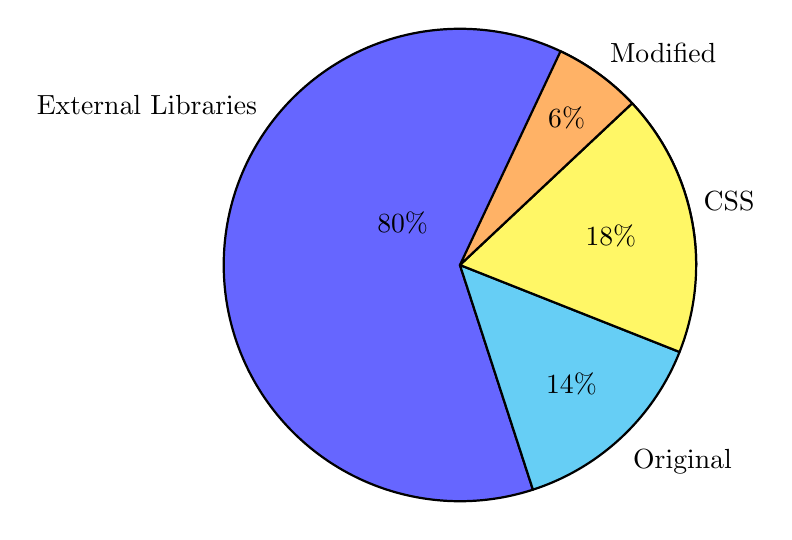
\begin{tikzpicture}
		\pie{80/External Libraries,  14/Original, 18/CSS, 6/Modified}
	\end{tikzpicture}
	\caption{sources of code}
	\label{overflow}
\endminipage\hfill
\minipage{0.45\textwidth}
	\centering
	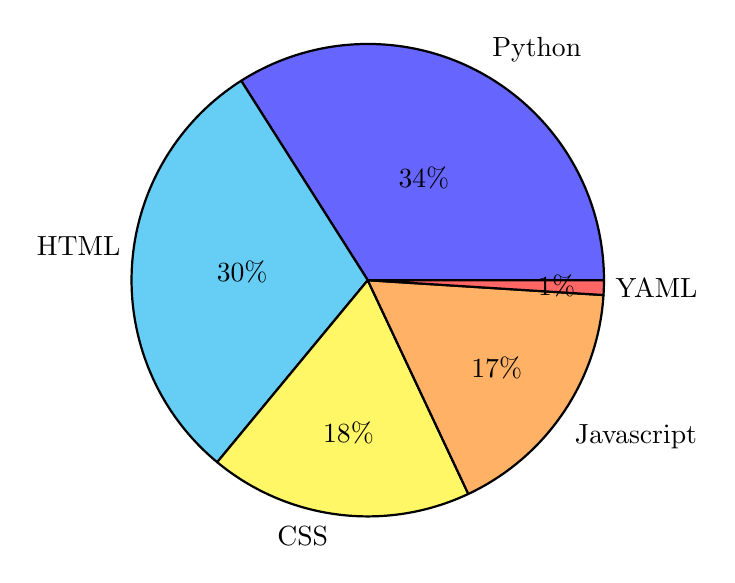
\begin{tikzpicture}
		\pie{34/Python, 30/HTML, 18/CSS, 17/Javascript, 1/YAML}
	\end{tikzpicture}
	\caption{lines of code per language}
	\label{overflow}
\endminipage
\end{figure}

{\em Figure 1} shows the distribution of the different sources of code sections, be it original code, modified code or code from external libraries.
{\em Figure 2} shows the distribution of lines of code between the different languages used throughout the coding of the application.


\newpage
\section{Brief overview of design and implementation}
For the Python back end portion of the application, Django was used. There were many reasons for this, each of which is outlined below.
Django is considered a heavyweight solution for short tasks, since files such as settings.py produce overheads; however, members of the group had used it before, and its template processing library is extremely useful. It also provides decent abstraction for handling pages (views). Thus, it was the obvious choice for use in this section of the application.
\\
!!!!NoSQL used for storage - Hayden or jamie know about this bit!!!! For scraping, Cron jobs (and other python files not included in Django) were used; these provided relatively simple implementations for features such as weekly email reminders for subscribed users, and such were utilised so the code was not written from scratch, saving time, effort and lines of code.
\\
Perhaps we could have a nice graphic that shows the different processes in our system? Not sure exactly what you want here
\\
Implementation of the front end was done using a combination of JavaScript, HTML and CSS, which included using a variety of external sources. JQuery was chosen due to its robust nature with respect to interacting with HTML elements, along with the fact that it is much more useful and effective for this type of application than plain JavaScript. d3 was used as a graphing library as it provides a very simple framework for creating extremely aesthetic graphics, so was implemented for the creation of graphs for episode ratings. The use of Bootstrap was due to its provision of fast prototyping of responsive websites - Bootflat is then an extension for Bootstrap, and is used to make the output of Bootstrap more aesthetic.

There is probably a bit more padding to be done here but I�ve bullshitted a fair amount anyway, just needs the NoSQL bit filled in and it should be alright.

\newpage	
\section{Critical evaluation of the prototype submitted}
The main aim of this project was to exhibit the group�s competency with both Python and JavaScript; as such, effort was made to effectively display this competency.

Were the prototype to be released to the public, the GAE likely would not be the best place to host the application. This is because of the probability of incurring significant, charges as the application is extremely data heavy and the GAE puts data usage limits in place. Furthermore, it was found that scraping large shows exceeded the memory usage of the app engine, as the XML parser consumed a large amount of memory when traversing large XML files. 

Additionally, there were a few features which were desirable, but with which there were problems including. Ideally, the calendar would display the times at which shows air; however, the API being used had no consistent time format which made this impossible. A page for each episode would also have been desirable, enabling users to post their comments about the show; however, this proved too time-consuming and did not justifiably demonstrate any greater competency with either Python or JavaScript. 

A consistent coding style was aimed for, with Python being documented using Sphinx. Additionally JavaScript was checked using JSHint in order to ensure the code was correct. However, this was only used as a guideline, as there are occasionally inconsistencies in the errors thrown by JSHint; as such, it was under the group�s discretion as to whether each error was heeded.

The group dynamic was extremely good - regular meetings were held each week in order to discuss issues and delegate tasks. While some disagreements arose, they were dealt with diplomatically and fairly, on occasion falling to group vote; as such, the work ethic and attitude of the group stayed positive and progress was made quickly and effectively.
\\
The application produced turned out extremely well; as, during its formulation, it was something the group felt would be useful, it was pleasing to see it flourish as a tool which would be used by each member. 
The process of creation was also very successful; using GitHub to publish, discuss and resolve issues provided a succinct method by which to fix bugs, add features and edit designs. These issues could be assigned to members, so completion was fast and effective, and the work could be spread between the group members based on skills and strengths.
\\
However, the initial planning of the work could have potentially been done better - as a result, a reasonable proportion of the work had to be done remotely over the Christmas break, which meant other commitments over this period also conflicted with getting the work done. Despite this, it was not an issue and the work was still completed effectively, and each group member committed to contributing and set aside time to make sure it was completed to the highest standard.
\\
During testing of the application, it was found that larger TV shows caused issues on the GAE during scraping; shows such as Emmerdale consist of a vast number of seasons and episodes, so scraping this enormous amount of data created problems. This was overcome, however, by not scraping each episode rating for shows with more than ten seasons, thus reducing the amount of data retrieved without removing any main functionality from the application. On top of this, there is the option to disable scraping for any given show through an admin account (i.e. one of the group members), so once it has been scraped once (and the information held persistently in the datastore) it is no longer necessary to scrape the show again, removing the need to retrieve such a large amount of data via scraping again.
\\
With hexagons being the main design choice, it was imperative they were done correctly and effectively within the code. Finding that there were issues with creating such shapes in CSS, Python-generated hexagons were opted for, and rendered for use in the application. This was extremely successful and made the process far simpler.
\\
To conclude, a highly successful application has been created, allowing users to search for, subscribe to and view statistics/air times for their favourite TV shows. It successfully demonstrates the group�s competency in both Python and JavaScript, whilst providing a useable service at the same time.

DO WE NEED THIS?
What would we do differently? 
Better planning - rather than diving straight into coding we couldve made lots of wireframes and a list of functionality and set deadlines and come up with class diagrams etc before implementing the program.


\end{document}
